\section{Classifying gamma-ray bursts}
In Exercise 6, we are asked to classify $\gamma$-ray bursts with logistic regression. $\gamma$-ray bursts can be either fast (classified as 1) or slow (classified as 0). 


Logistic regression is similar to linear regression, where we fit a model $$\hat{y} = h_\theta(\vec{x}) = \vec{\theta}^T \vec{x} + b$$ with parameters $\vec{\theta}$ and $b$ to features $\vec{x}$. The difference with linear regression is that we now use the sigmoid function as activation function, to limit the output between 0 and 1. The sigmoid function is defined as
\begin{equation}
\sigma(y) = \frac{1}{1+e^{-y}}
\end{equation}
It has the nice property that 
\begin{equation}\label{eq:derivsigm}
\frac{\partial }{\partial y} \sigma(y) = \sigma(y)(1-\sigma(y)),
\end{equation}
which allows us to calculate the derivative with already known values.
Thus the prediction function for logistic regression is
\begin{equation}
\hat{y} = h_\theta(\vec{x}) = \sigma( \vec{\theta}^T \vec{x} + b)
\end{equation}

We optimize the prediction function by minimizing the loss function. The loss function is defined as the binary cross-entropy loss function:
\begin{equation}
J(\theta) = -\frac{1}{m} \sum_{i=1}^{m} y_i \log(h_\theta(\vec{x}_i)) + (1-y_i) \log(1-h_\theta(\vec{x}_i))
\end{equation}
where $m$ is the number of training examples.

The loss function shall be minimized using gradient descent:
\begin{equation}
\theta_j = \theta_j - \alpha \frac{\partial J(\theta) }{\partial \theta_j}
\end{equation}
where $\alpha$ a hyperparameter called the learning rate. 
Using the property of the sigmoid function (Eq. \ref{eq:derivsigm}), the derivative of the loss function with respect to the parameters $\theta$ is then by
\begin{equation}
\frac{\partial J(\theta) }{\partial \theta_j} = \frac{1}{m} \sum_{i=1}^m (h_\theta(\vec{x_i}) - y_i) x_{i,j}
\end{equation}
where $x_{i,j}$ denotes the $j$-th feature of example $i$. 

In Python, we can vectorize all computations except the iterations of gradient descent by using matrices and dot products. We initialize $\theta$ as an ($n\times 1$) array and $X$ as an ($m\times$n) array. Because of \textit{NumPy} broadcasting $b$ can just be a float. The prediction of all training examples is then given by a dot product
\begin{equation}
\hat{y} = \sigma(X\cdot\theta + b)
\end{equation}
In this way, $\hat{y}$ is an $m\times 1$ array containing the predictions of all the training examples.

The back-propagation can also be vectorized, since we can calculate the derivatives as follows
\begin{equation}
\begin{split}
\frac{\partial J}{\partial b} = \frac{1}{m} \sum (\hat{y} - y) \\
\frac{\partial J}{\partial \theta} = \frac{1}{m} X^T \cdot (\hat{y}-y)
\end{split}
\end{equation}
where $y$ is now the ($m\times 1$) array containing the true labels. In this setup $\frac{\partial J}{\partial \theta}$ is an $n\times 1$ array containing the derivatives with respect to the $\theta$ array. 

We choose to standardize all features to have 0 mean and unit variance. For this standardization, we ignore the missing values. After standardization, we make sure that all missing values are set to the mean of the data, thus zero in this case. For every column where we adjust the missing values, we add another column that contains 1's where the value was initially missing and 0's where the value was not missing. This allows the network to distinguish between missing values and actual values. We split the initial set into a training and test set with ratio 75:25. 

As is indicated in the code, and the output of the code, there are a lot of missing values for most of the features. For this reason we have chosen to drop the last three feature columns as by far most values were missing for these columns and thus including these features would not be very useful. 

The full code that deals with missing values and does logistic regression in a vectorized way with gradient descent is given below.

\lstinputlisting[]{question6.py}

This script produces the following outputs:
\lstinputlisting[language={}]{q6output.txt}

In Figure \ref{fig:fig59}, we have plotted the value of the (binary cross-entropy) loss function, to show that the gradient descent algorithm has converged to optimal values of $w$ and $b$. Figures \ref{fig:fig54} and \ref{fig:fig55} show the predictions on the training and test set. As the output of the code shows, the accuracy is 0.78 on the training set and 0.81 on the test set, thus only marginally better than the ZeroR prediction of predicting everything as the most abundant class. Figures \ref{fig:fig56} to \ref{fig:fig58} explore why this is the case a little bit further. From inspecting these 2D projected plots, we can see that no clear regions can be found where the bursts are short as opposed to long. Therefore, it is very hard to perform better than the ZeroR prediction of classifying everything as long. This is worsened by the fact that for all features except redshift, most of the values are missing, as is indicated from the values that have a feature of 0 now. Combining features only makes sense if both features are not missing so effectively we only have very little features to work with.


The network now uses the redshift, star formation rate and mass of the host galaxy as first and second order features. We have decided to include the second order features as it is very clear from Figures \ref{fig:fig56} to \ref{fig:fig58} that a first order model will not be able to distinguish the short from the long bursts. A second order model does not perform great either, but it is at least better than the ZeroR prediction of predicting everything as a long burst. We see that the network is not overfitting because the network has a similar performance on the training set and the test set. 

\begin{figure}[ht]\centering
\begin{minipage}[t]{.5\textwidth}
\centering
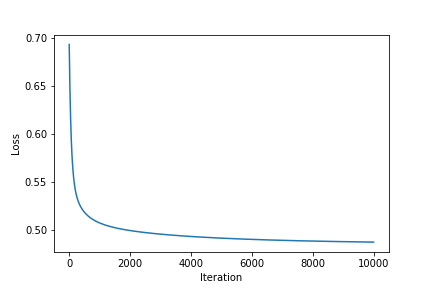
\includegraphics[width=1.0\linewidth]{./plots/q6_1.png}
\captionsetup{width=0.8\linewidth}
\captionof{figure}{Logistic regression predictions on the training set. 1 indicates a fast burst and 0 indicates a slow burst.}
\label{fig:fig54}
\end{minipage}%
\begin{minipage}[t]{.5\textwidth}
\centering
\includegraphics[width=1.0\linewidth]{./plots/q6_2.png}
\captionsetup{width=0.8\linewidth}
\captionof{figure}{Logistic regression predictions on the training set. 1 indicates a fast burst and 0 indicates a slow burst.}
\label{fig:fig55}
\end{minipage}%
\end{figure}

\begin{figure}[ht]\centering
\begin{minipage}[t]{.5\textwidth}
\centering
\includegraphics[width=1.0\linewidth]{./plots/q6_10.png}
\captionsetup{width=0.8\linewidth}
\captionof{figure}{2D projection of two features from the full dataset showing the predicted labels and actual labels.}
\label{fig:fig56}
\end{minipage}%
\begin{minipage}[t]{.5\textwidth}
\centering
\includegraphics[width=1.0\linewidth]{./plots/q6_20.png}
\captionsetup{width=0.8\linewidth}
\captionof{figure}{2D projection of two features from the full dataset showing the predicted labels and actual labels.}
\label{fig:fig57}
\end{minipage}%
\end{figure}

\begin{figure}[ht]\centering
\begin{minipage}[t]{.5\textwidth}
\centering
\includegraphics[width=1.0\linewidth]{./plots/q6_21.png}
\captionsetup{width=0.8\linewidth}
\captionof{figure}{2D projection of two features from the full dataset showing the predicted labels and actual labels.}
\label{fig:fig58}
\end{minipage}%
\begin{minipage}[t]{.5\textwidth}
\centering
\includegraphics[width=1.0\linewidth]{./plots/q6_loss.png}
\captionsetup{width=0.8\linewidth}
\captionof{figure}{Value of the binary cross-entropy loss function as a function of iteration of gradient descent.}
\label{fig:fig59}
\end{minipage}%
\end{figure}


